\Chapter{Tesztelés}

\Section{Használat}
A program használata egyszerű. Futtatás után a weboldalon kiválasztjuk a feldolgozandó fájlt. Innentől a program automatikusan működik. Ezután ki lehet választani a menüsávban a kívánt menüpontokat, amik átirányítanak a megfelelő oldalakra. Az első menüpont az architektúra, a második a kód oldal, harmadik a szimuláció. A kezdőoldalra a Szakdolgozatra kattintva lehet visszajutni. A kód oldalon a Gannt diagram elemeire kattintva lehet az egyes kódsorokat jobban megvizsgálni. A szimuláció oldalon lehet az aritmetikát vizsgálni, valamint saját szimulációt készíteni. Saját szimulációhoz útmutató a mellékelt Instruction Guide.txt és a Custom Instructions Example.txt

\Section{Tesztek}
A program az indulást követően szinte valós idejű, a szimulációra és a hardware szolgáltatásokra kell esetekben várni 1-2 másodpercet. Memória igény felső korlátja 160MB, tárhely igény 2 MB.

A program működése képernyőképeken át látható:

\begin{figure}[h]
\centering
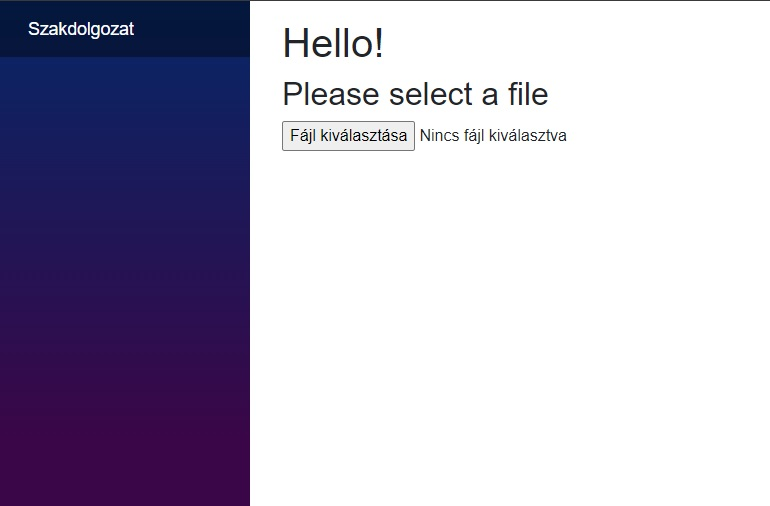
\includegraphics[scale=0.7]{images/Start.jpg}
\caption{Webalkalmazás kezdő állapota}
\label{fig:start}
\end{figure}

\begin{figure}[h]
\centering
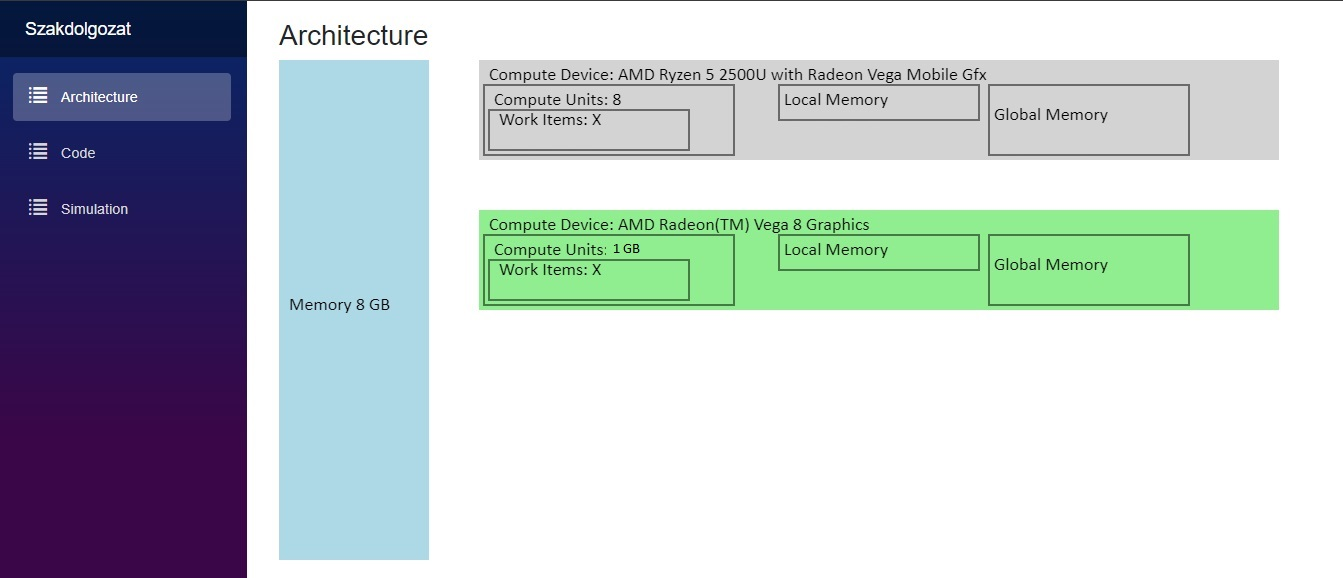
\includegraphics[scale=0.3]{images/Architecture.jpg}
\caption{Architekture oldal}
\label{fig:arch}
\end{figure}

\begin{figure}[h]
\centering
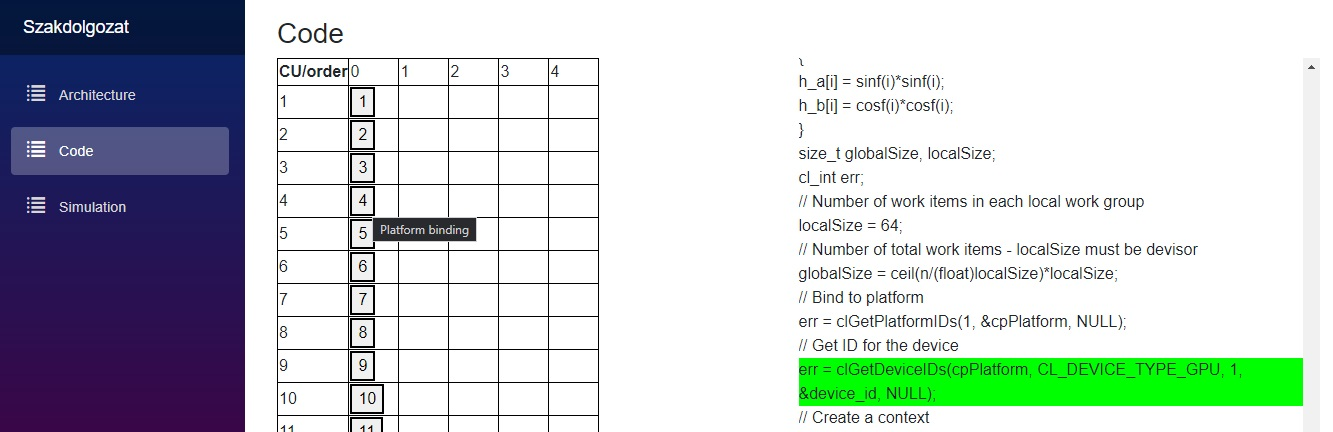
\includegraphics[scale=0.3]{images/Code.jpg}
\caption{Code oldal}
\label{fig:code}
\end{figure}

\begin{figure}[h]
\centering
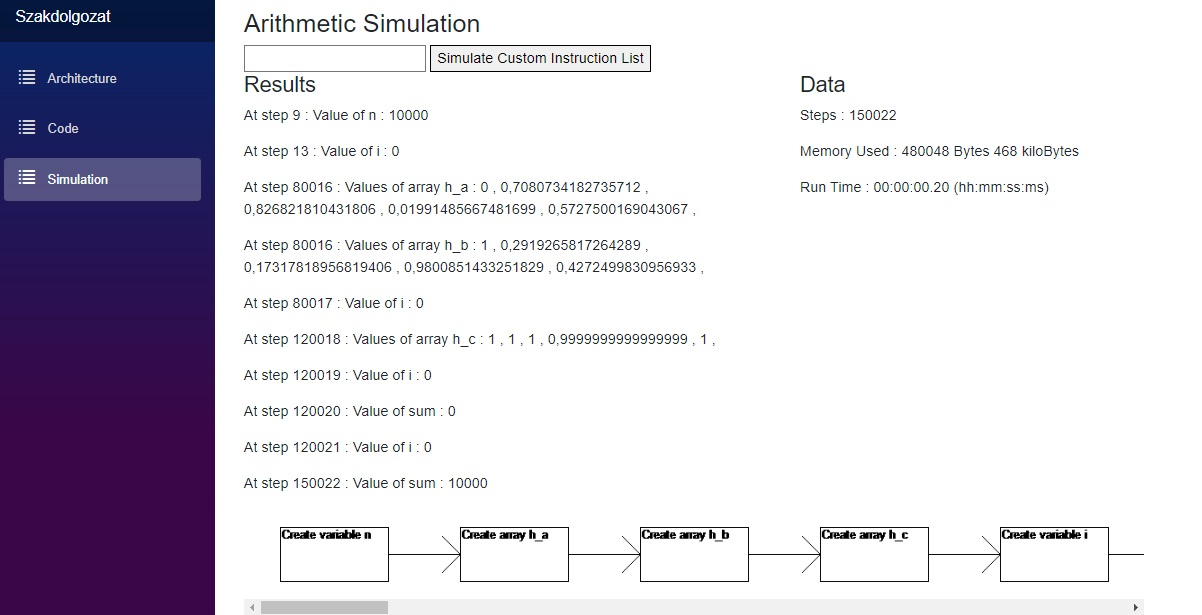
\includegraphics[scale=0.4]{images/Simulation.jpg}
\caption{Simulation oldal}
\label{fig:sim}
\end{figure}